\documentclass[../thesis.tex]{subfiles}

\begin{document}

\chapter{Real World Testing}

\section{Aim}

Verifying the the proposed system is working well with real devices on a small scale.

\section{Setup} % Things to do before the experiment.

The solar power generation setup is documented in the figure \ref{fig:realworldsensing}. In summary, the solar panel generates electricity, which is measured by the input sensor and fed into the converter. After converting to the desired voltage, the electricity is measured by the output sensor and stored in the battery. Additionally, there is an inverter that converts the DC electricity from the battery to AC. The electricity is then used to power the load and the microcontroller where the load in the experimental setup is a portable air conditioning unit. The real world setup is shown in the figure \ref{fig:realworld1} and \ref{fig:realworld2} and it is functionally equivalent to the setup in figure \ref{fig:realworldsensing}.

\begin{figure}[!ht]
	\centering
	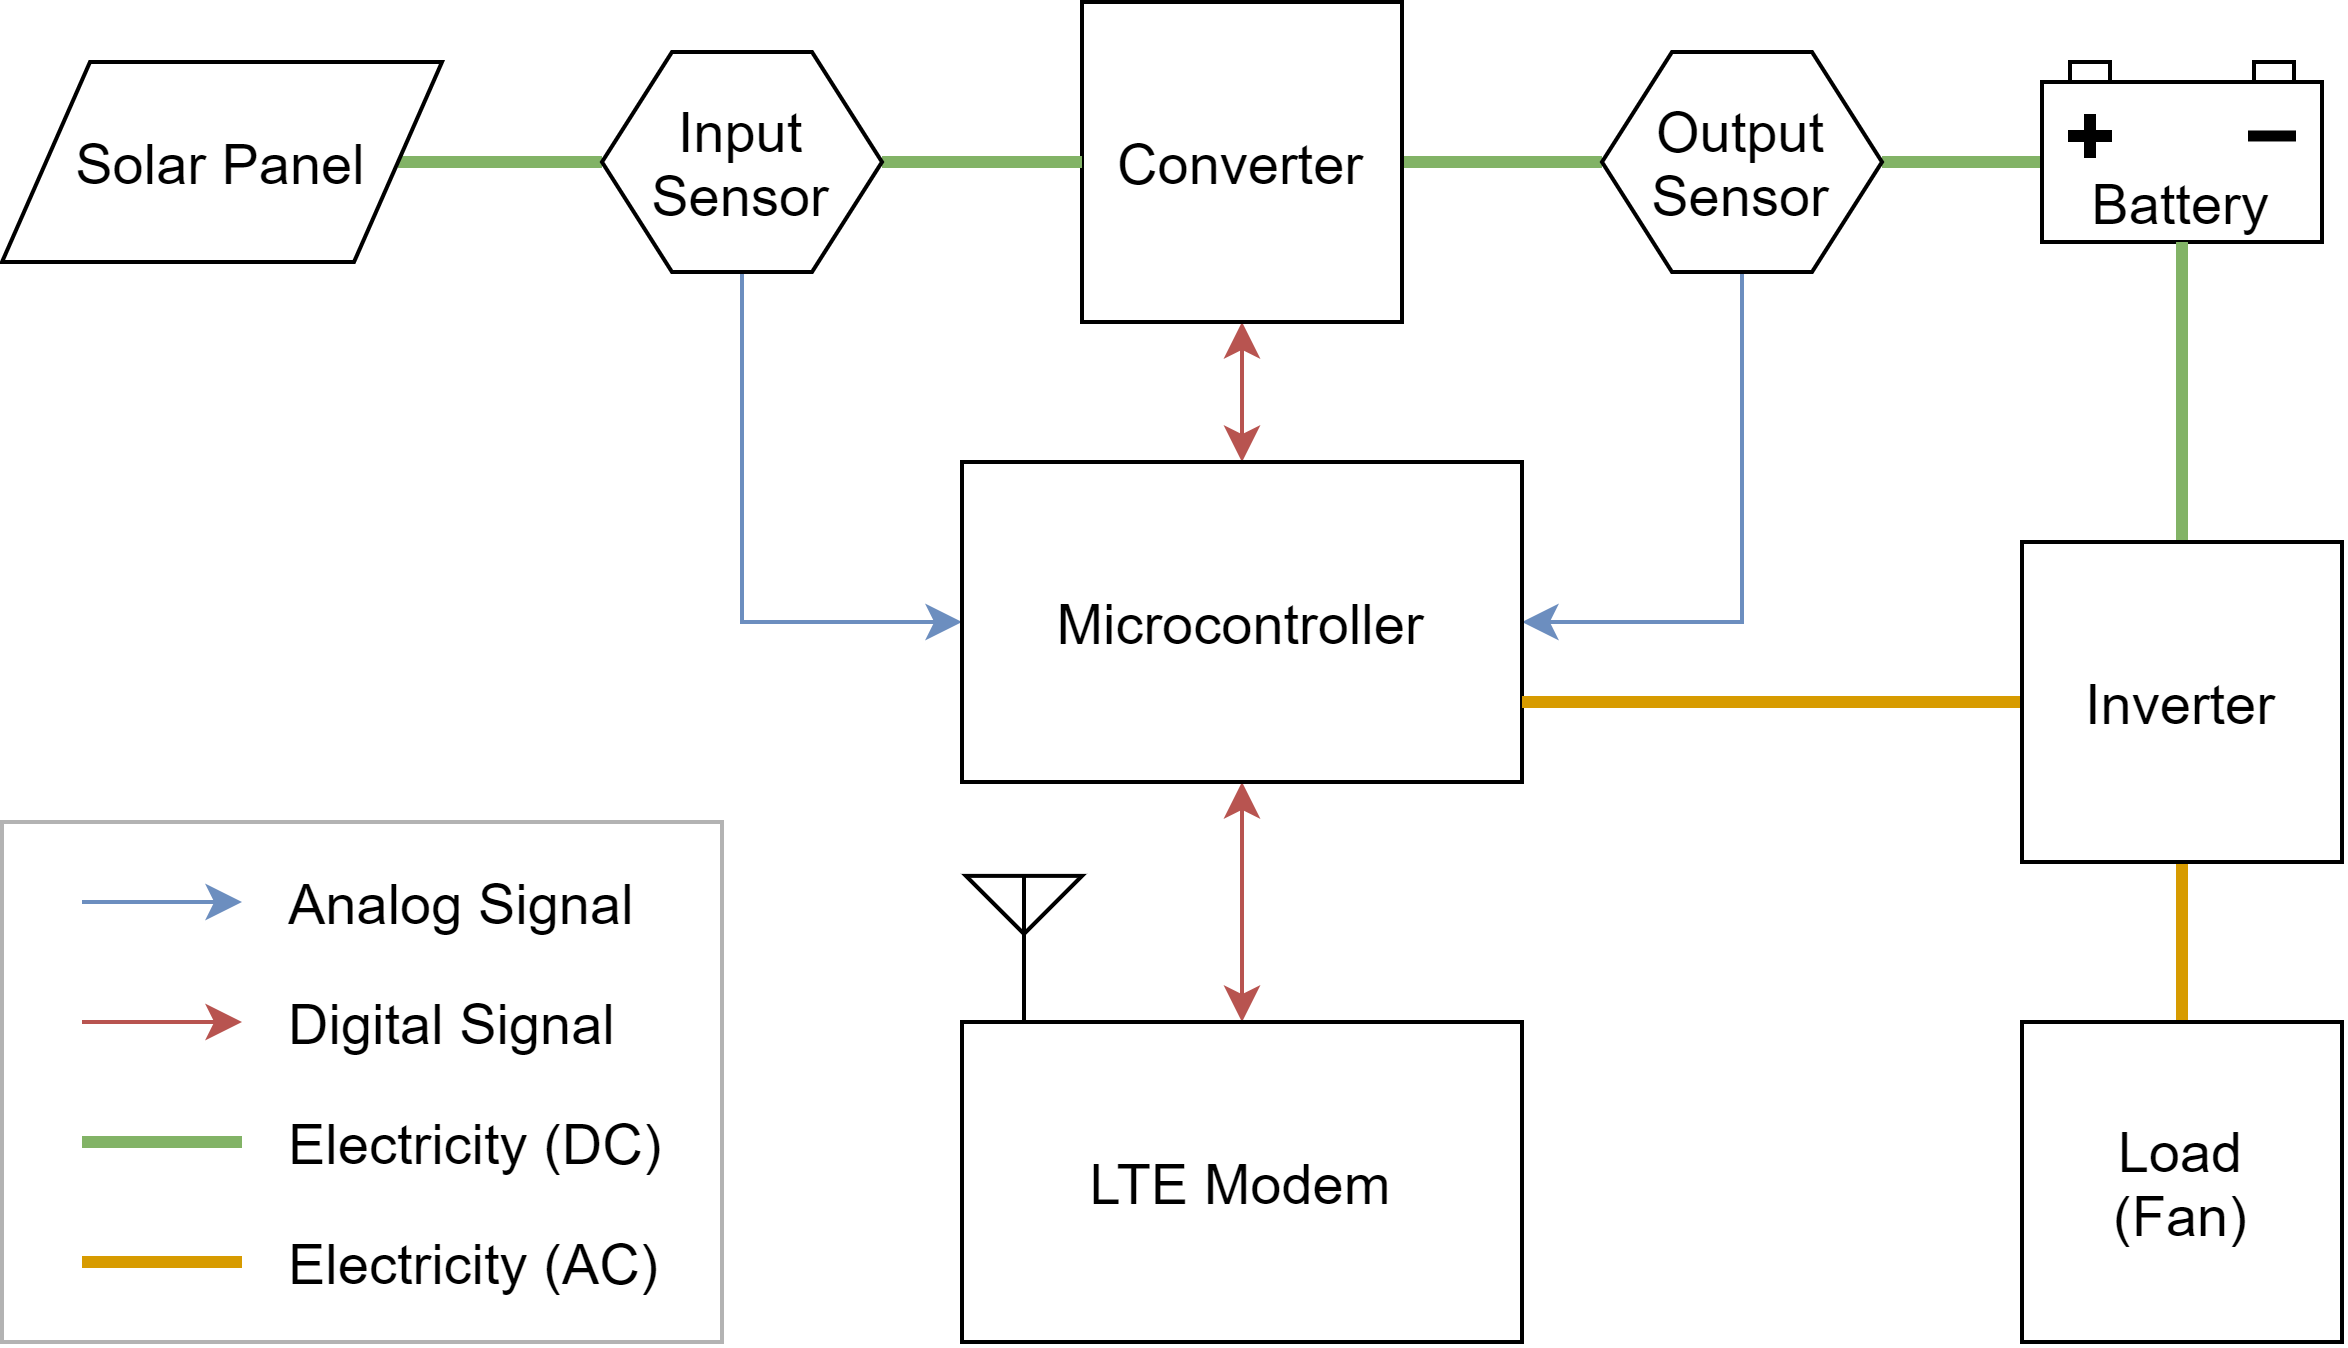
\includegraphics[width=\linewidth]{c6-sensing.png}
	\caption{The experimental setup (Schematic)}
	\label{fig:realworldsensing}
\end{figure}

The proposed system is deployed to an Elastic Compute Cloud (Amazon EC2) instance of type T2.Micro and the components are running inside Docker Containers. Finally, the firewall is configured to allow public access to the frontend and backend servers. 

A sim card with a 4G data plan is inserted into the microcontroller and the modem is connected to the microcontroller through the mini-PCIe slot. The antenna must be attached to the MAIN connector of the modem to communicate with any LTE base station. Additionally, the external power cable supplies power to the LTE modem, and the board power cable supplies power to the microcontroller, both cables must be connected to the board for the controller and modem to work properly together. The setup is shown in the figure \ref{fig:realworld4}. 

Configurations of the sim card is either set ahead of firmware compile time or detected automatically from the mobile service provider.

\begin{figure}[!ht]
	\centering
	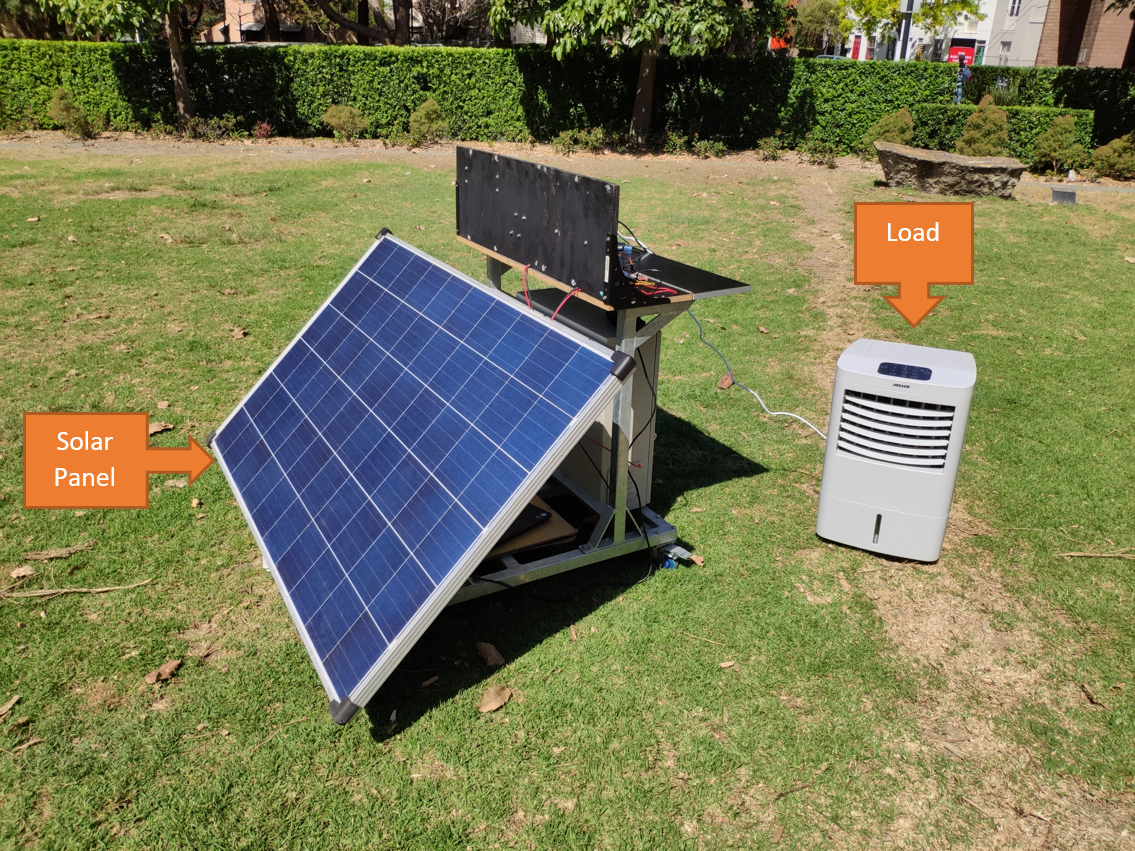
\includegraphics[width=0.8\linewidth]{realworld1.png}
	\caption{The experimental setup (front)}
	\label{fig:realworld1}
\end{figure}

\begin{figure}[!ht]
	\centering
	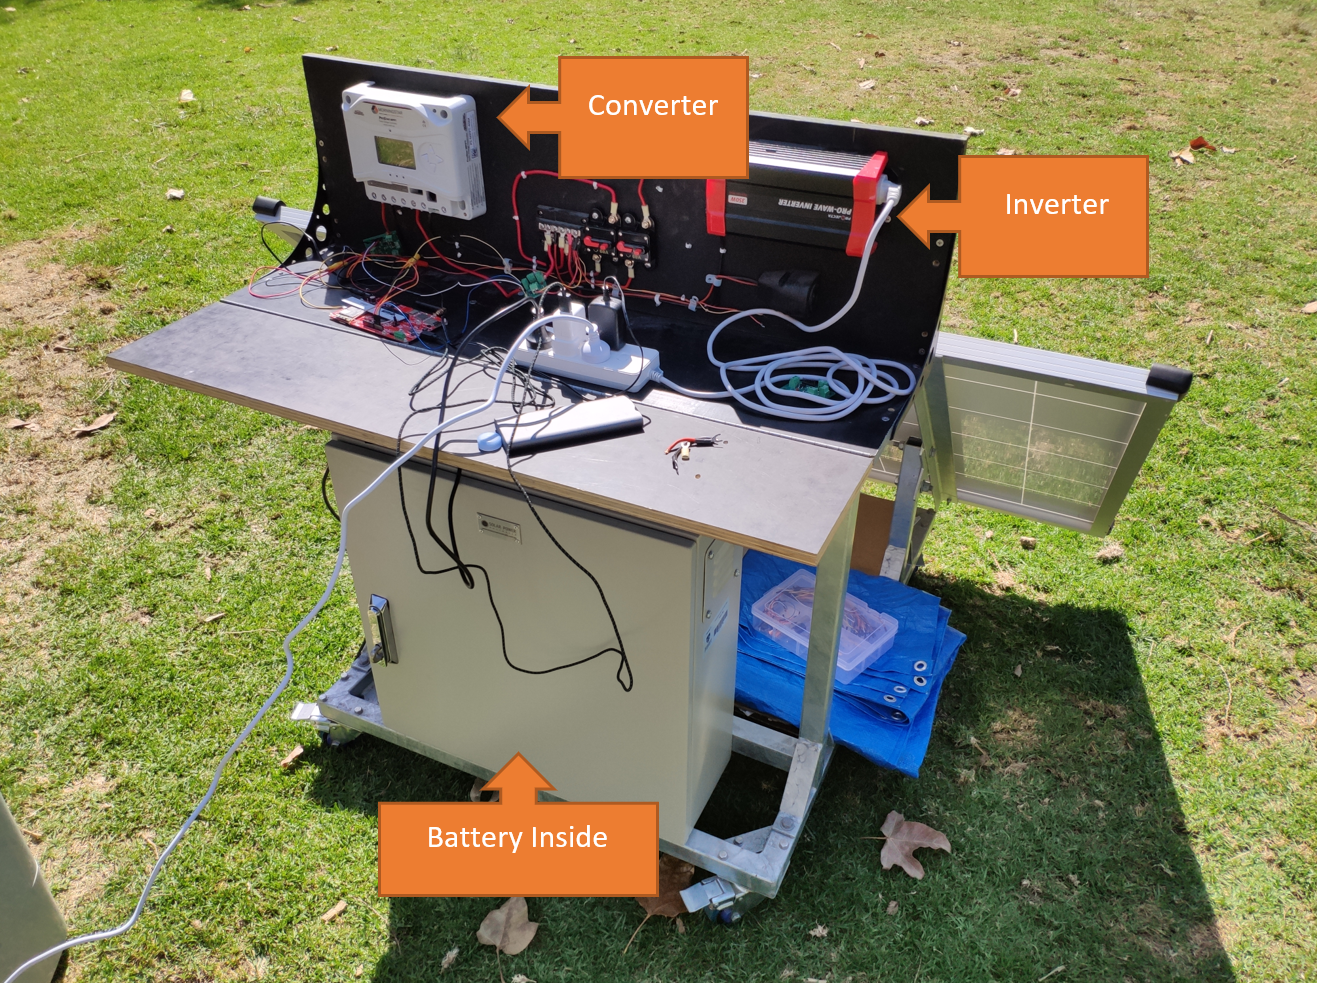
\includegraphics[width=0.8\linewidth]{realworld2.png}
	\caption{The experimental setup (back)}
	\label{fig:realworld2}
\end{figure}

\begin{figure}[!ht]
	\centering
	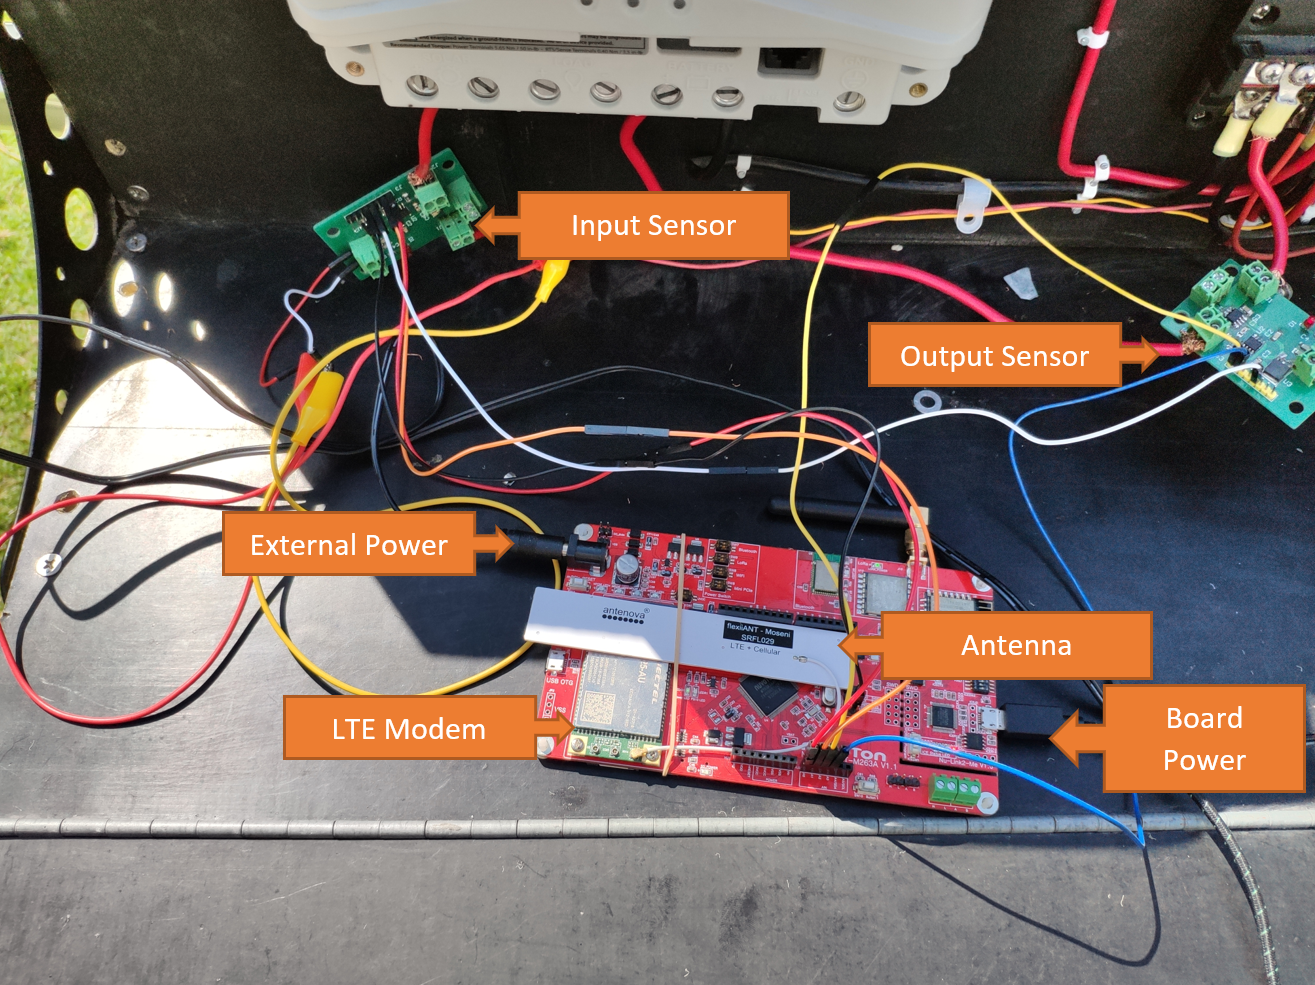
\includegraphics[width=0.8\linewidth]{realworld4.png}
	\caption{The experimental setup (controller)}
	\label{fig:realworld4}
\end{figure}

\section{Procedures} % Things to do during the experiment



\section{Analysis}


\end{document}